\subsection{1. Prototype - Staying Within the Lines}

The first prototype needs to be able to drive, turn and brake. Furthermore, it needs to be able to combine these mechanisms to stay within the lines of the track. To drive the bus it'll use a LEGO Servo Motor to provide forwards and backwards capabilities, which will be done by connecting it to the rear wheels. The speed consistency of the bus is not important in this prototype, however driving at a higher speed allows for testing the capabilities of the sensors and their processing speed.
%however the Servo Motor should be set at \todo{80\%}, to make sure the bus can drive at high speed and still stay within the lines at all times, but the actual speed are not to be measured.

The front wheels are used for turning and will be powered by a LEGO Servo Motor. It should be able to turn the same amount of degrees to both sides, however, there is no requirement for a specific turning angle for this prototype. A thing to note is that the track for the bus should be designed such that the bus can perform the turn within the lines.

To prevent crashes the prototype should have obstacle detection by having a LEGO ultrasonic sensor placed at the very front of the bus in a fixed position. The sensor should detect obstacles \todo{5?} cm ahead and \todo{30?} degrees to both sides. If it predicts that a collision might occur, the bus should stop immediately, overriding both the driving and turning procedures. When this obstacle is no longer a hindrance, it will return to its normal state.  % Later prototype should be able to get out of this situation

For the prototype to stay within the lines of the track, two LEGO NXT Light Sensors should be placed at the very front, one on each side to detect the lines on both sides. The sensors should aim directly at the ground with a distance of \todo{0.5?} cm to the ground. \info{Are we sure we won't be using the camera?}

The bus itself should be formed like a long rectangle so that it gets the form of a bus. It should have \todo{1:3?} length to width ratio.

\subsubsection{Track requirements}
The designed track for this prototype can be seen on figure \ref{Track1Layout}. The layout of the track is quite simple and only contain some of the requirements described in section \ref{Requirements}. The reason for this is to only test the features of this prototype and as such is designed uniquely for this prototype.

The requirements for the track has therefore been limited to:
\cite{DriveingCurves}
\begin{itemize}
  \item One lane, with a width of the minimal turning space requirement.
  \item 6\% extra lane width on each side.
  \item 180 degrees turn with the minimal length and width.
  \item Small turns.
  \item Pedestrian crossing for testing obstacle detection.
\end{itemize}

\begin{figure}[H]
    \label{Track1Layout}
    \centering
    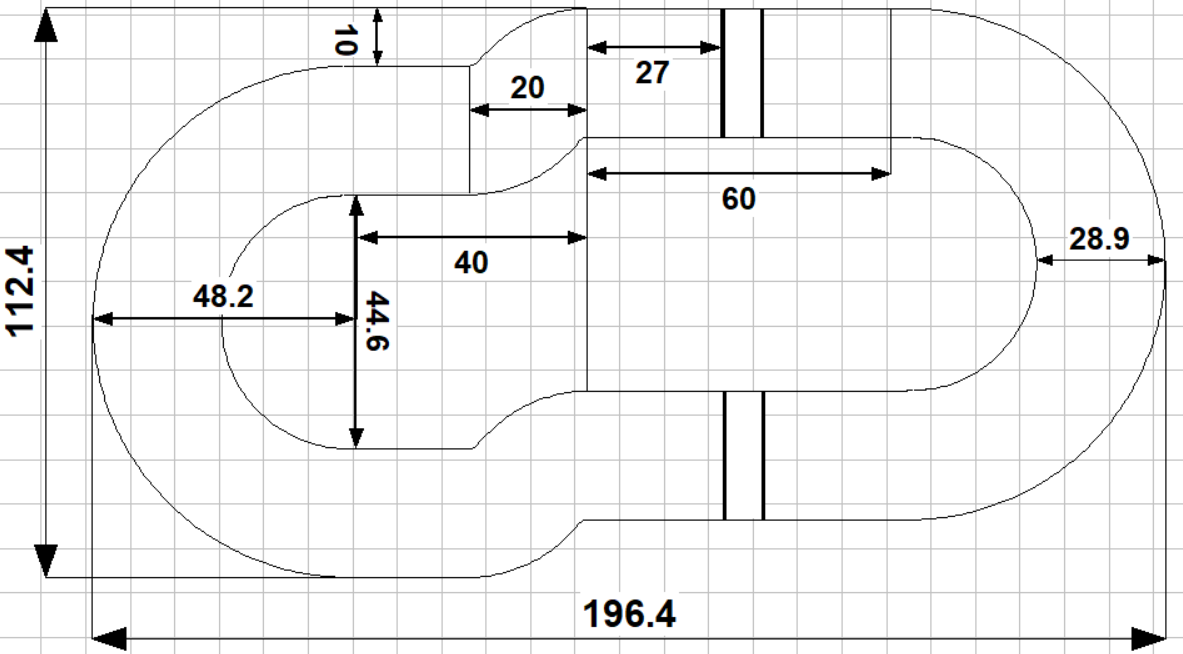
\includegraphics[width=0.8\textwidth]{Images/Tracks/Track1.PNG}
    \caption{Track 1 Layout}
\end{figure}

\todo{Insert Final layout}







